\documentclass{article}

\usepackage[margin=0.75in, headheight=35pt, includehead, includefoot]{geometry}

\usepackage{fancyhdr}
\usepackage[T1]{fontenc}
\usepackage[shortlabels]{enumitem}
\usepackage{graphicx}
\graphicspath{ {./} }
\usepackage[export]{adjustbox}
\usepackage{booktabs}
\usepackage{forest}
\usepackage{listings}
\lstset{escapeinside={(*@}{@*)}, showstringspaces=false}

\setlength{\parindent}{4em}
\setlength{\parskip}{1em}

\pagestyle{fancy}
\rhead{Alex Kitsul\\230134210\\April 1, 2022}

\begin{document}
\thispagestyle{empty}
\begin{center}
\topskip0pt
\vspace*{\fill}
\Huge Alex Kitsul\\
\Huge 230134210\\
\Huge CPSC 450\\
\Huge Assignment 6 - Report\\
\Huge April 1\\
\vspace*{\fill}
\end{center}
\pagebreak

\section*{Psedocode}
\begin{lstlisting}
main:
    k <- from file
    m <- from file
    points <- from file as format (x, y)

    centers <- LloydsAlgorithm(points, k)
    print(centers)
	
LloydsAlgorithm(data, k):
    centers = random k centers
    clusters = dict() with center indexes as keys and empty lists as values

    while(!converged):
        for point in data:
            closest_center = None
            for center in centers:
                if(distance(point, center) < distance(point, closest_center)):
                    closest_center = center

            clusters[closest_center].append(point)

        for center in clusters:
            new_center = mean of all points in cluster
            if centers are the same:
                converged = True
            centers[center] = new_center
            clusters[center] = []

    return centers
\end{lstlisting}

\pagebreak

\section*{Program Code}
\textbf{\underline{LloydsAlgorithm.py}}
\lstinputlisting[language=Python]{../LloydsAlgorithm.py}

\pagebreak

\section*{Examples with Output}
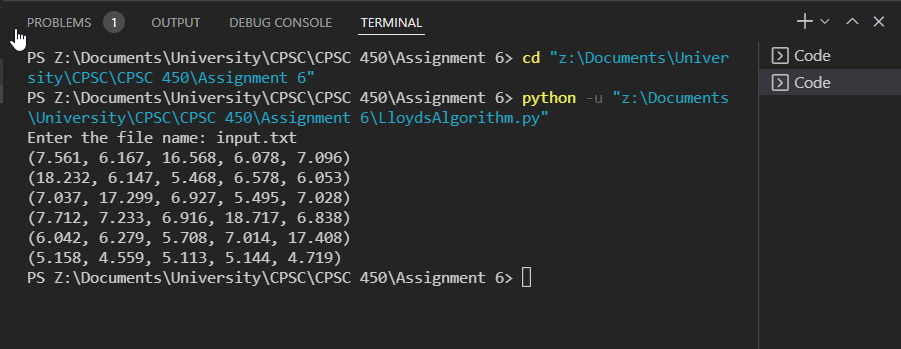
\includegraphics[scale=0.55]{input.png}\\
% \includegraphics[scale=0.55]{input_2.png}\\
% \includegraphics[scale=0.55]{input_3.png}\\

\end{document}
